%-------------------------------------------------------------------------------
% CAPITOLO 23
%-------------------------------------------------------------------------------
\chapter{Lezione 23}
\label{capitolo_23}
\textit{23/05/2026}

\section{Modello di Massima Entropia}
La distribuzione di probabilità $P(S)$ di massima entropia può essere espressa in una forma simile a quella di Boltzmann:

\begin{equation} \label{eq:ch23_1}
P(S) = \frac{e^{-\sum_{\mu} \lambda_{\mu} O^{\mu}(S)}}{Z}
\end{equation}

dove $O^{\mu}(S)$ sono certe osservabili che misuriamo dai dati, $\lambda_{\mu}$ sono i moltiplicatori di Lagrange, $Z$ è la funzione di partizione.
I moltiplicatori di Lagrange $\{\lambda_{\mu}\}$ sono determinati imponendo che i valori predetti delle osservabili eguaglino i valori ottenuti sperimentalmente:

\begin{equation} \label{eq:ch23_2}
\langle O^{\mu}(S) \rangle = \langle O^{\mu} \rangle_{EXP}
\end{equation}

dove $\langle O^{\mu}(S) \rangle$ è il valore predetto dal modello, e $\langle O^{\mu} \rangle_{EXP}$ è il valore medio sperimentale dell'osservabile.
Il modello che otteniamo dipende dalle osservabili che scegliamo. È ragionevole iniziare con osservabili semplici, che possiamo stimare nel miglior modo possibile sperimentalmente, e poi verificare a posteriori se il modello ottenuto ha un qualche potere predittivo. Se non è abbastanza buono, si possono aggiungere altre osservabili.


\section{Applicazione alle Reti Neurali: Modello a 1 Punto}
Consideriamo il caso dei neuroni. La configurazione microscopica $S$ è l'insieme di tutte le variabili di attività $S_i$ che specificano se un neurone $i$ sta scaricando (firing) o meno ($S_i \in \{-1,1\}$).
Come osservabili $O^{\mu}(S)$, consideriamo inizialmente i singoli valori di firing $S_i$. Quindi, misuriamo sperimentalmente l'attività media di ciascun singolo neurone $\langle S_i \rangle_{EXP}$.
Sperimentalmente, se misuriamo l'attività di singoli neuroni (o elettrodi) nel tempo, dividiamo l'asse temporale in piccoli intervalli $d\tau$ (dell'ordine dei millisecondi). L'intervallo deve essere abbastanza piccolo da non avere eventi doppi al suo interno.
L'attività media sperimentale del neurone $i$ è calcolata come:

\begin{equation} \label{eq:ch23_3}
\langle S_i \rangle_{EXP} = \frac{1}{t_{TOT}} \sum_{a=1}^{N_{TOT}} S_i(t_a)
\end{equation}

Questo viene fatto per tutti i neuroni, ottenendo un insieme di osservabili $\{\langle S_i \rangle_{EXP}\}$ per $i=1, \dots, N$.
In questo caso, l'indice $\mu$ delle osservabili corrisponde all'indice $i$ del neurone.
Rinominiamo i moltiplicatori di Lagrange $\lambda_i \rightarrow -h_i$. La scelta del segno negativo è convenzionale per ottenere una forma simile a un modello di Ising ferromagnetico.
La distribuzione di probabilità diventa:

\begin{equation} \label{eq:ch23_4}
P(S) = \frac{e^{\sum_i h_i S_i}}{Z[\{h_i\}]}
\end{equation}

Questa è una forma simile a quella di Boltzmann (Boltzmann-like).
Per determinare i parametri $h_i$, imponiamo la condizione:

\begin{equation} \label{eq:ch23_5}
\langle S_i \rangle = \langle S_i \rangle_{EXP} \quad \forall i=1, \dots, N
\end{equation}

Per un modello di spin indipendenti (con $S_i \in \{-1,1\}$ e $\beta=1$), la magnetizzazione locale $m_i = \langle S_i \rangle$ è data da:

\begin{equation} \label{eq:ch23_6}
m_i = \tanh(h_i)
\end{equation}

Quindi, abbiamo $\langle S_i \rangle_{EXP} = \tanh(h_i)$. Invertendo questa relazione, otteniamo $h_i$:

\begin{equation} \label{eq:ch23_7}
h_i = \text{arctanh}(\langle S_i \rangle_{EXP})
\end{equation}

Una volta misurati gli $\langle S_i \rangle_{EXP}$, possiamo calcolare gli $h_i$ e quindi il modello è completamente specificato.


\section{Controllo della Predittività del Modello a 1 Punto}
Una volta ottenuto un modello, dobbiamo verificare se è significativo e se ha potere predittivo. Ci sono due modi principali per farlo.

\subsection*{Variazione dell'Entropia}
L'idea del modello di massima entropia è trovare il modello con la maggiore entropia possibile, consistente con i dati. L'entropia $S(P)$ è data da:

\begin{equation} \label{eq:ch23_8}
S(P) = -\sum_S P(S) \ln P(S)
\end{equation}

Se assumiamo $P(S) = \text{costante}$ (=nessuna informazione sperimentale), l'entropia è massima ($S_{max}$). Questo corrisponde a un sistema completamente casuale.
Quando introduciamo l'informazione sperimentale (ad esempio, le medie $\langle S_i \rangle_{EXP}$, dette "informazione a 1 punto"), ci aspettiamo che l'entropia diminuisca. Questo perché non tutte le configurazioni sono equiprobabili; solo quelle che producono i valori specifici delle osservabili misurate dovrebbero essere campionate da questa distribuzione.
Il punto è capire di quanto diminuisce l'entropia:
\begin{itemize}
    \item Se l'entropia diminuisce molto, significa che l'informazione sperimentale fornita al modello è molto rilevante.
    \item Se l'entropia diminuisce poco, significa che l'informazione è povera e non molto significativa.
\end{itemize}

Nel caso delle reti neurali con solo informazione a 1 punto, si osserva che l'entropia diminuisce un po', ma non in modo sostanziale rispetto all'entropia massima del caso completamente casuale. Questo suggerisce che l'informazione a 1 punto potrebbe non essere sufficiente.

\subsection*{Predizione di Osservabili di Ordine Superiore}
Un secondo modo per testare il modello è fare una predizione con la distribuzione di probabilità ottenuta e verificare se la predizione è corretta rispetto ai dati. Avendo fornito al modello informazioni a 1 punto (medie $\langle S_i \rangle$), possiamo provare a vedere cosa predice il modello per osservabili di ordine successivo, come le correlazioni a 2 punti $\langle S_i S_j \rangle$.
Per il modello a 1 punto, che è un modello non interagente (la probabilità si fattorizza sui singoli siti $i$), la predizione per la correlazione tra due unità $i$ e $j$ è:

\begin{equation} \label{eq:ch23_9}
\langle S_i S_j \rangle = \langle S_i \rangle \langle S_j \rangle
\end{equation}

Poiché abbiamo imposto $\langle S_i \rangle = \langle S_i \rangle_{EXP}$, la predizione del modello è:

\begin{equation} \label{eq:ch23_10}
\langle S_i S_j \rangle = \langle S_i \rangle_{EXP} \langle S_j \rangle_{EXP}
\end{equation}

Possiamo misurare sperimentalmente le correlazioni $C_{ij}^{EXP} = \langle S_i S_j \rangle_{EXP}$ dai dati:

\begin{equation} \label{eq:ch23_11}
\langle S_i S_j \rangle_{EXP} = \frac{1}{t_{TOT}} \sum_{a=1}^{N_{TOT}} S_i(t_a) S_j(t_a)
\end{equation}

Si confrontano quindi i valori $\langle S_i S_j \rangle$ con i valori $\langle S_i S_j \rangle_{EXP}$. Se il modello è buono, i punti su un grafico "teorico vs sperimentale" dovrebbero trovarsi vicino alla bisettrice.

\vspace{0.5cm}
\noindent\fbox{%
    \parbox{\dimexpr\linewidth-2\fboxsep-2\fboxrule\relax}{%
        \textbf{!!}\\
        Per una rete di neuroni, si trova che questo non è il caso. Questo significa che una rete di neuroni non si comporta come un'aggregazione di neuroni indipendenti, ma si influenzano a vicenda. La correlazione non è semplicemente data dal prodotto delle attività individuali; c'è qualcosa di più.\\
        Questo implica che l'informazione a 1 punto non è sufficiente.
    }%
}
\vspace{0.5cm}


\section{Modello a 2 Punti}
Poiché il modello a 1 punto non è sufficientemente predittivo, il passo successivo è includere anche informazioni sulle coppie di neuroni.
Le osservabili ora includono sia le attività medie dei singoli neuroni $\langle S_i \rangle_{EXP}$ sia le correlazioni tra coppie di neuroni $\langle S_i S_j \rangle_{EXP}$. I moltiplicatori di Lagrange associati a $\langle S_i \rangle$ sono ancora $-h_i$, mentre quelli associati a $\langle S_i S_j \rangle$ li chiamiamo $-J_{ij}$. (Il segno meno è per convenzione, per far assomigliare il modello a un modello di Ising con campi e interazioni ferromagnetiche).
La distribuzione di probabilità diventa:

\begin{equation} \label{eq:ch23_12}
P(S) = \frac{e^{\sum_i h_i S_i + \sum_{ij} J_{ij} S_i S_j}}{Z[\{h_i\}, \{J_{ij}\}]}
\end{equation}

Questa distribuzione ha la forma di un modello di Ising con campi esterni $h_i$ e interazioni $J_{ij}$ tra gli spin (neuroni). A priori, tutti i $J_{ij}$ possono essere diversi.
Per specificare completamente il modello, dobbiamo trovare i valori degli $h_i$ e dei $J_{ij}$. Questo si fa imponendo le condizioni:

\begin{equation} \label{eq:ch23_13}
\langle S_i \rangle = \sum_S S_i P(S) = \langle S_i \rangle_{EXP}
\end{equation}

\begin{equation} \label{eq:ch23_14}
\langle S_i S_j \rangle = \sum_S S_i S_j P(S) = \langle S_i S_j \rangle_{EXP}
\end{equation}

Risolvere questo sistema di equazioni analiticamente è molto più complicato rispetto al caso a 1 punto, perché il modello di Ising con $J_{ij}$ generici non è risolvibile analiticamente. Pertanto, questo problema deve essere risolto numericamente.
La procedura numerica, in breve, consiste nel:

\begin{enumerate}
    \item Iniziare con una stima per gli $h_i$ e $J_{ij}$.
    \item Con questi parametri, eseguire una simulazione (es. Monte Carlo) del modello per calcolare $\langle S_i \rangle$ e $\langle S_i S_j \rangle$.
    \item Confrontare questi valori con quelli sperimentali $\langle S_i \rangle_{EXP}$ e $\langle S_i S_j \rangle_{EXP}$.
    \item Aggiornare iterativamente i parametri $h_i$ e $J_{ij}$ per ridurre la discrepanza tra i valori predetti e quelli sperimentali, fino a quando i valori predetti numericamente sono sufficientemente vicini ai valori reali.
\end{enumerate}

Bialek e collaboratori hanno eseguito questa procedura. Hanno prima provato un modello a singolo sito, si sono resi conto che era sbagliato, e poi hanno aggiunto l'informazione sulle coppie.
Quando si include l'informazione a 2 punti (le correlazioni $\langle S_i S_j \rangle_{EXP}$), si osserva una diminuzione significativa dell'entropia rispetto al modello a 1 punto. Questo suggerisce che l'informazione sulle coppie è molto rilevante.
Successivamente, si possono controllare le predizioni del modello per osservabili di ordine ancora superiore, come le correlazioni a 3 punti $\langle S_i S_j S_k \rangle_{EXP}$.
Se si aggiungesse l'informazione a 3 punti al modello, l'entropia diminuirebbe ulteriormente, ma si osserva che questa diminuzione è molto piccola rispetto al salto ottenuto passando da 1 a 2 punti. Questo andamento (grande salto di entropia a un certo livello di informazione, e poi piccole diminuzioni per livelli superiori) indica che l'informazione più rilevante è stata catturata.

La conclusione principale è che l'informazione sulle coppie (pairwise) è quella cruciale da includere in un modello di attività neuronale. Le interazioni di ordine superiore sono meno rilevanti. Dire che a livello statistico l'informazione importante è pairwise può anche essere interpretato come dire che le interazioni sono prevalentemente pairwise. Quindi assumere che i neuroni interagiscano a coppie è una buona approssimazione.
Questi modelli di tipo Ising, una volta determinati i $J_{ij}$, possono presentare frustrazione (come nei vetri di spin), ma si è osservato che nei sistemi neuronali la frustrazione non è estrema come nei vetri di spin canonici. C'è un dibattito in corso sul fatto che le reti neurali tendano ad operare vicino a un punto critico.


\section{Proteine}
Le proteine sono eteropolimeri. Un polimero è una sequenza di gruppi molecolari chiamati monomeri; un eteropolimero è un polimero in cui questi gruppi possono essere diversi.
Nelle proteine, i monomeri sono gli amminoacidi.
La struttura generale di un amminoacido è la seguente:

\begin{figure}[h!]
\centering
% 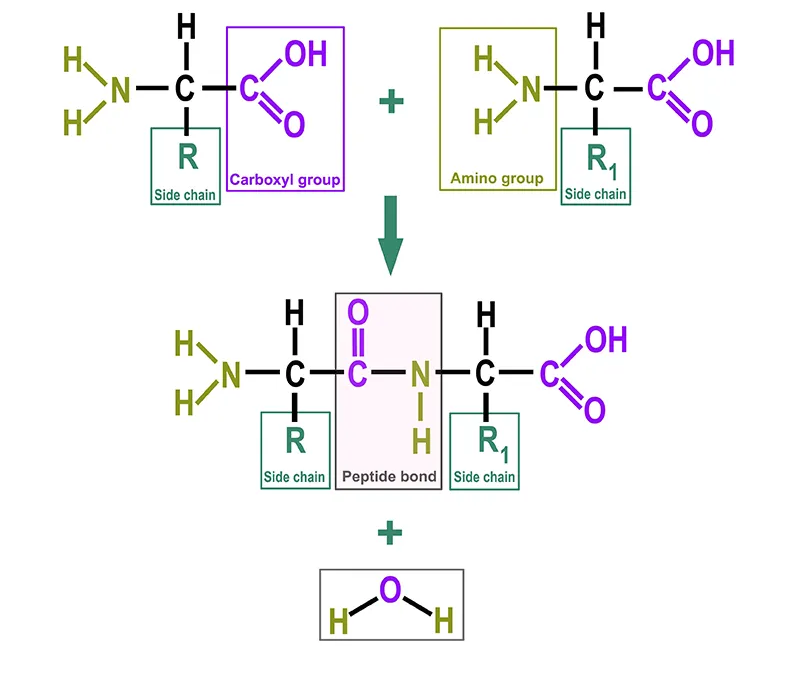
\includegraphics[width=0.4\textwidth]{pics/23_1.png} % INSERIRE QUI LO SCHEMA DELL'AMMINOACIDO
\caption{Struttura generale di un amminoacido. $R$ rappresenta il gruppo residuo (catena laterale).}
\label{fig:ch23_1}
\end{figure}

Dove $R$ è il residuo che definisce il tipo di amminoacido. Esistono 20 tipi comuni di residui, e quindi 20 tipi di amminoacidi.
Gli amminoacidi si legano tra loro attraverso un legame peptidico, che si forma tra il gruppo carbossilico di un amminoacido e il gruppo amminico di un altro, con l'eliminazione di una molecola d'acqua.

Una catena di amminoacidi costituisce la struttura primaria di una proteina. La lunghezza tipica di una proteina è di circa 200 amminoacidi.
Con 20 tipi di amminoacidi e una lunghezza di 200, il numero di sequenze possibili è $20^{200}$, un numero enorme. Tuttavia, solo una frazione molto piccola di queste sequenze possibili corrisponde a proteine funzionali osservate in natura.
Oltre alla sequenza (struttura primaria), sono fondamentali per la funzione di una proteina le sue strutture secondaria, terziaria e quaternaria. Queste descrivono come la catena polipeptidica si ripiega (folds) nello spazio tridimensionale. Le proteine funzionali si trovano tipicamente in una specifica conformazione ripiegata (native state).
Possiamo rappresentare una sequenza proteica come $S = \{S_1, S_2, \dots, S_L\}$, dove $L$ è la lunghezza della proteina ($L \approx 200$) e $S_i \in \{1, \dots, 20\}$ specifica il tipo di amminoacido nella posizione $i$-esima della catena.
La struttura tridimensionale può essere definita specificando le coordinate spaziali di ciascun amminoacido: $\Sigma = \{\vec{r}_1, \vec{r}_2, \dots, \vec{r}_L\}$.

Nel ripiegamento, amminoacidi che sono distanti lungo la catena possono venire a trovarsi vicini nello spazio tridimensionale. Se questi amminoacidi "vicini nello spazio" hanno affinità chimica, possono formare interazioni non covalenti (come legami idrogeno) che stabilizzano la struttura tridimensionale. Questo legame tra sequenza e struttura è cruciale per capire perché solo alcune sequenze sono funzionali.
Le proteine sono spesso divise in famiglie. Proteine appartenenti alla stessa famiglia tendono a ripiegarsi nello stesso modo (stessa struttura tridimensionale) e ad avere funzioni biologiche simili, pur potendo avere sequenze amminoacidiche significativamente diverse (fino al 40\% di differenze). Questo indica che, sebbene la sequenza sia importante, c'è una certa flessibilità.
Per modellizzare una proteina, si può definire un'energia $E(S, \Sigma)$ che dipende sia dalla sequenza $S$ che dalla struttura $\Sigma$. Un'espressione generale per l'energia $E(\{\vec{r}_i\})$ (per una data sequenza $S$) include:

\begin{itemize}
    \item \textbf{Un termine elastico} che mantiene la connettività della catena polipeptidica:
\end{itemize}
\begin{equation} \label{eq:ch23_15}
E_{chain} = \frac{k}{2} \sum_i (\left|\vec{r}_{i+1} - \vec{r}_i\right| - l_0)^2
\end{equation}
dove $l_0$ è la distanza di legame tipica tra amminoacidi adiacenti e $k$ è una costante elastica elevata.

\begin{itemize}
    \item \textbf{Un termine di interazione} tra coppie di amminoacidi $(i,j)$ non necessariamente adiacenti nella sequenza ma che possono trovarsi vicini nello spazio:
\end{itemize}
\begin{equation} \label{eq:ch23_16}
E_{int} = \frac{1}{2} \sum_{i \neq j} V(S_i, S_j) U(\left|\vec{r}_i - \vec{r}_j\right|)
\end{equation}
dove $V(S_i, S_j)$ dipende dal tipo di amminoacidi $S_i$ e $S_j$, e $U(\left|\vec{r}_i - \vec{r}_j\right|)$ è un potenziale che dipende dalla loro distanza.

\begin{itemize}
    \item \textbf{Un termine di volume escluso}, che tiene conto del fatto che due amminoacidi non possono occupare lo stesso spazio. Questo è un termine entropico che può essere rappresentato come un'energia effettiva.
\end{itemize}
\begin{equation} \label{eq:ch23_17}
E_{vol} = \frac{1}{2} \sum_{i \neq j} V_0(\left|\vec{r}_i - \vec{r}_j\right|)
\end{equation}

La forma complessiva dell'energia può essere scritta come:

\begin{equation} \label{eq:ch23_18}
E(\{\vec{r}_i\}) = \frac{k}{2}\sum_{i}(\left|\vec{r}_{i+1}-\vec{r}_i\right|-l_0)^{2} + \frac{1}{2}\sum_{i \neq j}V(S_i,S_j)U(\left|\vec{r}_i-\vec{r}_j\right|) + \frac{1}{2}\sum_{i \neq j}V_0(\left|\vec{r}_i-\vec{r}_j\right|)
\end{equation}

Il paesaggio energetico (energy landscape) di una proteina è fondamentale. Se $V(S_i, S_j)$ fosse una variabile casuale, si otterrebbe un paesaggio energetico simile a quello di un vetro di spin, con molti minimi locali di energia comparabile. Questo non è desiderabile per una proteina, che tipicamente deve raggiungere uno stato nativo ben definito in modo efficiente.
Si pensa che le proteine funzionali abbiano un paesaggio energetico a "imbuto" (funnel), con un minimo globale ben pronunciato che corrisponde allo stato nativo, guidando il ripiegamento verso di esso.


\section{Modello Semplificato}
Per studiare la relazione tra sequenza, struttura ed energia, sono stati proposti modelli semplificati. Uno di questi è il modello HP (Idrofobico-Polare).
\begin{itemize}
    \item La lunghezza della catena è ridotta: $L=27$.
    \item Ci sono solo due tipi di amminoacidi: Idrofobici (H) e Polari (P). Quindi $S_i \in \{H, P\}$.
    \item Gli amminoacidi sono confinati su un reticolo, ad esempio un reticolo cubico 3D. Per $L=27$, la struttura più compatta possibile è un cubo $3 \times 3 \times 3$.
    \item Si definiscono energie di interazione tra amminoacidi adiacenti sul reticolo (non legati covalentemente lungo la catena): $E_{HH}$, $E_{PP}$, $E_{HP}$.
\end{itemize}

Per favorire la formazione di un nucleo idrofobico (con gli amminoacidi H all'interno della proteina, lontani dal solvente acquoso, e i P sulla superficie), si scelgono le energie in modo che l'interazione H-H sia la più favorevole:

\begin{equation} \label{eq:ch23_19}
E_{PP} > E_{HP} > E_{HH} 
\end{equation}

L'energia di una data sequenza $S$ in una data conformazione $\Sigma$ è $E(S, \Sigma)$, data dalla somma delle energie di contatto tra amminoacidi vicini non legati covalentemente.

Studiando lo spazio delle sequenze e delle strutture per questi modelli semplificati, si possono trarre alcune conclusioni:
\begin{itemize}
    \item Non tutte le strutture compatte sono lo stato fondamentale (ground state, GS) di una qualche sequenza. Alcune strutture non sono mai la conformazione di minima energia per nessuna sequenza.
    \item Alcune sequenze hanno uno stato fondamentale degenere, cioè possono ripiegarsi in molte strutture diverse con la stessa energia minima. Questo non è desiderabile per una proteina che deve avere una funzione specifica legata a una struttura specifica.
    \item D'altra parte, la maggior parte delle strutture sono "poco designable": sono lo stato fondamentale di pochissime sequenze. Sarebbe quindi molto improbabile "trovare" una sequenza che si ripiega specificamente in una di queste strutture.
    \item Esiste però un piccolo numero di strutture "altamente designable": sono lo stato fondamentale di un numero molto elevato di sequenze diverse. Queste strutture sono "attrattori" nello spazio delle sequenze.
\end{itemize}

Se si traccia un grafico del numero di strutture che sono il ground state per un dato numero di sequenze, si osserva che un elevato numero di diverse conformazioni strutturali è generato da un esiguo numero di sequenze. Inversamente, solo poche strutture uniche sono associate a un vasto insieme di sequenze. Ciò significa che la maggior parte delle strutture sono "poco designable", mentre poche sono "altamente designable", cioè realizzabili da molte sequenze diverse.
L'idea è che le proteine reali corrispondano a queste strutture altamente designable.

\begin{figure}[h!]
\centering
% 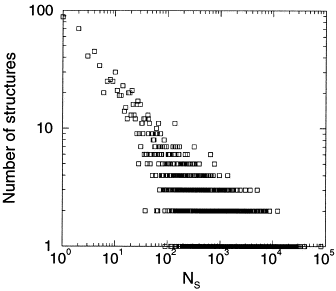
\includegraphics[width=0.6\textwidth]{pics/23_2.png} % INSERIRE QUI IL GRAFICO DELLA DESIGNABILITY
\caption{Grafico della \textit{designability}: sull'asse verticale il numero di strutture differenti, sull'asse orizzontale il numero di sequenze per le quali una data struttura $\Sigma$ rappresenta lo stato di minima energia.}
\label{fig:ch23_2}
\end{figure}

Queste strutture altamente designable spesso presentano particolari simmetrie e sono più stabili. La stabilità è intesa come un ampio gap energetico tra lo stato fondamentale e il primo stato eccitato. Un grande gap significa che la proteina è robusta a piccole perturbazioni e rimane nel suo stato nativo.
Questo approccio aiuta a capire la drastica riduzione dal numero enorme di sequenze possibili al numero relativamente piccolo di strutture proteiche osservate e funzionali.
